\chapter{\introductionname}\label{chap:introduction}
\section{Research Background and Context}
Computation is \textit{everywhere}. 
 This statement is not just a catchy phrase but a reflection of our current reality, 
 shaped by the accelerated development of information technology. 
 Indeed, computation has been seamlessly integrated into our everyday lives, 
 so much so that it often goes unnoticed. 
%
Its \emph{ubiquitous} presence transcends traditional boundaries, 
 not just in professional settings but also in our homes, transportation systems, 
 and even our bodies, as evidenced by \emph{wearable} technologies. 
% 
This phenomenon is most evident in the explosion of \ac{iot} devices. 
 According to recent statistics~\footnote{\url{https://www.statista.com/statistics/1183457/iot-connected-devices-worldwide/}}, 
 there are currently over 15 billion IoT devices globally, 
 and this number is expected to surpass 30 billion by the year 2030.

The widespread adoption of computational technologies has ushered in a transformative phase for the IT landscape, 
 starting from the \emph{edge} of the network where connected devices are becoming more sophisticated and efficient. 
 These edge devices are not merely passive data collectors but are now capable of \emph{localized} computation  (thus \emph{cyber-physical}), storage, and analytics. 
Moving towards the core, 
 \emph{cloud} infrastructures are also undergoing significant metamorphosis. 
 Traditional centralized data centres are evolving into a more distributed,
 decentralized, and dynamic architecture to meet the ever-changing demands of users and applications.

In this light, the term \emph{edge-cloud continuum} aptly encapsulates the current IT landscape. 
 It symbolizes a \emph{fluid} environment where the edge and the cloud are not isolated silos but exist as two poles on a spectrum. 
 Between these poles lies a multitude of intermediate layers, 
 comprising \emph{fog computing}, micro data centres, and hybrid cloud solutions, among others. 

This fluid computational landscape is endorsed by contemporary theories like  ubiquitous~\cite{DBLP:journals/sigmobile/Weiser99}, pervasive
 ~\cite{DBLP:journals/computer/SahaM03}, and collective~\cite{DBLP:journals/computer/Abowd16}.
%
These paradigms collectively herald an era where computation 
 is not confined to specific devices but emerges as an integrated capability across a vast, 
 interconnected ecosystem in which a vast arrays of simple devices interact in a decentralized fashion, 
 harnessing their collective, might to accomplish intricate tasks often far beyond the capability of individual units. 
%
Drawing from natural systems, 
 it is striking how these intricate computational networks mimic the complex collective behaviours seen in nature. 
 For example, certain social insects, like ants and bees, display remarkable examples of resilient, effective, and efficient self-organizing systems. 
 Such natural phenomena serve as powerful metaphors for understanding and conceptualizing the self-organizing propensities within computational systems.
 
These observations have culminated in the formulation of the concept of \acp{cpsw}, 
 an ensemble of \emph{heterogeneous} computational entities deeply integrated with the physical world. Unlike monolithic systems, \acp{cpsw} leverages diversity—both in terms of device capabilities and functionalities—to achieve collective objectives. 
 This heterogeneous nature enriches the system's adaptability, robustness, and overall performance, thereby enabling it to solve problems in a more nuanced manner.
%
Instances of \acp{cpsw} are becoming increasingly prevalent and varied, 
 seen not only in the realm of swarm robotics but also in human crowd dynamics and in the burgeoning field of IoT devices. 
 In each of these cases, the core principles remain consistent: the employment of self-organizing mechanisms to achieve collective goals in an efficient, resilient, and \emph{adaptable} manner.

\section{Overview and Contribution}
Addressing the engineering challenges of \ac{cpsw} requires innovative approaches, 
 as traditional device-centric and bottom-up methodologies fall short. 
The complexities involved in these swarms stem from a myriad of factors, 
 including the nuanced interaction between local and global dynamics, 
 the intricacies associated with distributed control systems, 
 the evolving landscape of IT architectures, and significant scalability considerations.
%
Given these multifaceted challenges, 
 this thesis introduces a comprehensive \emph{language-based} approach (i.e., solution built around a programming model) that incorporates robust models, 
 cutting-edge techniques, and pioneering algorithms. 
 The objective is to streamline the design and deployment of self-organizing behaviours in \acp{cpsw} that are both \emph{predictable} and \emph{adaptable}. 
This is achieved by integrating established manual design methodologies, namely aggregate computing, 
 with cutting-edge advances in machine learning, such as \ac{marl}. 
%
This \emph{hybrid} approach aims to harness the strengths of both paradigms to create a more robust, efficient, and scalable \ac{cpsw} framework.

The research underpinning this work draws from a wide array of interdisciplinary fields, 
 such as swarm robotics, multi-agent systems, collective adaptive systems, aggregate computing, and multi-agent reinforcement learning. 
By synthesizing insights from these diverse domains, 
 the proposed approach aims to offer a holistic solution for the effective engineering and deployment of Cyber-Physical Swarms.
\subsection{Problem statement}
The current state-of-the-art solutions in both automatic and manual design are limited in handling the complexities arising from the collective intelligence of \ac{cpsw}. 
 While the former may offer gold-standard solutions through a ``learn-by-doing'' approach, 
 they often struggle to generalize across different scenarios. 
 On the other hand, manual solutions may excel in modularity and declarative design but frequently fall short when it comes to managing complex environmental conditions.
Therefore, what is the optimal model for engineering such applications? 
 Does a hybrid approach that combines both automatic and manual design offer any advantages? 
 Are there specific requirements for \ac{cpsw} that differentiate them from other collective adaptive systems?
 Lastly, how does the engineering of these applications influence the design process for collective controllers?
\subsection{Contributions}

The thesis contributes to an area called ``language-based engineering,'' where models, algorithms, machine learning solutions, and tools are constructed around a specific programming language within a given context. As a case in point, this thesis focuses on aggregate computing because it aligns closely with the needs of designing applications for Cyber-Physical Social Systems (CPSWs). 
This can be largely attributed to the self-organizing characteristics of aggregate computing, which are independent of system size. Additionally, its high-level programming model facilitates the design of collective applications.

In this regard, the thesis explores both hybrid aggregate computing and standard engineering approaches, which is reflected in its structure. Specifically, our contributions toward a hybrid approach include:
\begin{enumerate}
    \item developing a comprehensive roadmap for integrating aggregate computing with machine learning,
    \item introducing a collective program synthesis method to establish robust self-organizing behaviours,
    \item proposing a distributed scheduling solution to accelerate the convergence of collective structures expressed through aggregate computing,
    \item presenting a novel multi-agent reinforcement learning technique, termed ``field-informed reinforcement learning,'' designed to create robust distributed controllers for large-scale computations, and
    \item creating a tool called ScaRLIB, which supports hybrid aggregate computing by combining state-of-the-art deep learning libraries with the aggregate computing toolchain.
\end{enumerate}
While, contributions toward standard engineering approaches include:
\begin{enumerate}
    \item introducing a novel programming language called FRASP, which is designed to facilitate the engineering of self-organizing behaviors in CPSWs,
    \item developing of a set of `swarm-like' API for coordinated movement, distributed sensing and sensing-based clustering
    \item A novel architecture for deployment on the edge-cloud continuum through a multi-tier pulverized architecture.
\end{enumerate}
\begin{figure}
    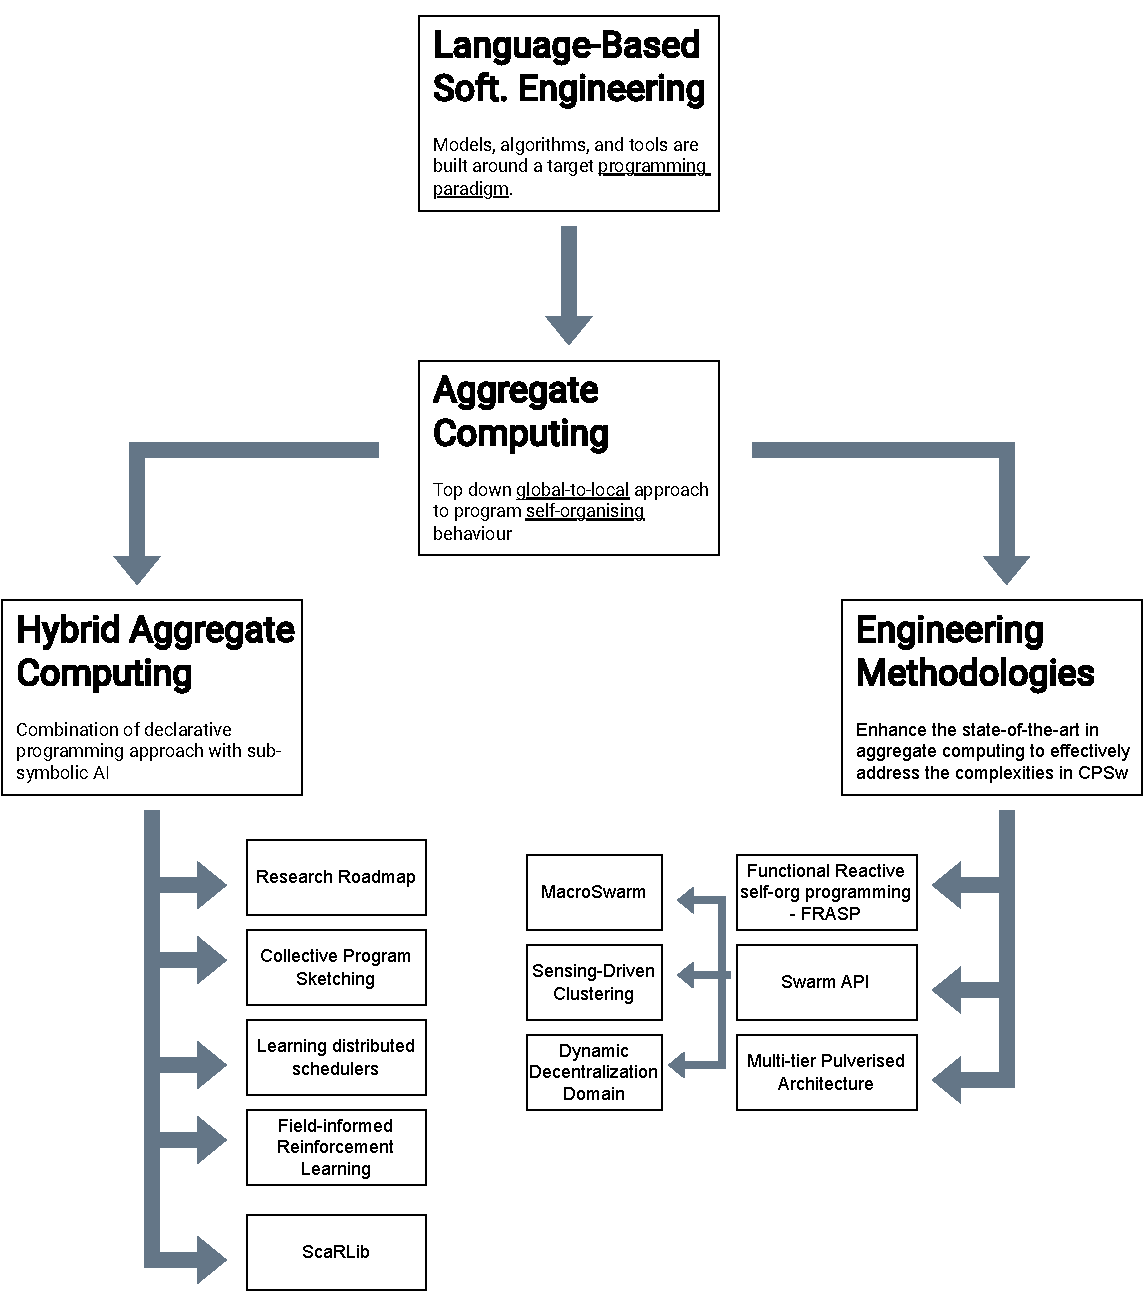
\includegraphics[width=\textwidth]{chapters/img/contribution-visual.drawio.pdf}
    \caption{Graphical overview of the thesis contributions.}
\end{figure}
\section{Thesis structure}
This thesis is organized as follows.

\Cref{chap:introduction} provides an overview of the research background and context, 
 and outlines the thesis structure and contributions.

\Cref{part:background} presents the theoretical foundations of this work.

\Cref{part:learning} introduces the contribution of the proposed hybrid approach for learning in \acp{cpsw}.

\Cref{part:engineering} discuss the contribution w.r.t. the engineering aspect of \acp{cpsw}.
\printbibliography[title=References]

\section{Publication List}

